\documentclass[18pt]{beamer}
\usepackage[utf8]{inputenc} % for the umlauts
\usepackage{subfigure}

\beamertemplatenavigationsymbolsempty
%% SLIDE FORMAT

% use 'beamerthemekit' for standard 4:3 ratio
% for widescreen slides (16:9), use 'beamerthemekitwide'

\usepackage{templates/beamerthemekit}
\usepackage{stackengine}
\usepackage{graphicx}
\usepackage{verbatim}
\usepackage{tikz}
\usepackage{tikz-uml}
\usepackage{caption}
\captionsetup[figure]{labelformat=empty}% redefines the caption setup of the figures environment in the beamer class.

% \usepackage{templates/beamerthemekitwide}

\setcounter{tocdepth}{1}

%% TITLE PICTURE

% if a custom picture is to be used on the title page, copy it into the 'logos'
% directory, in the line below, replace 'mypicture' with the 
% filename (without extension) and uncomment the following line
% (picture proportions: 63 : 20 for standard, 169 : 40 for wide
% *.eps format if you use latex+dvips+ps2pdf, 
% *.jpg/*.png/*.pdf if you use pdflatex)

%\titleimage{mypicture}

%% TikZ INTEGRATION

% use these packages for PCM symbols and UML classes
 \usepackage{templates/tikzkit}
	\usepackage{templates/tikzuml}

% the presentation starts here

\usepackage[absolute,overlay]{textpos}
\usepackage{csquotes}
%\usepackage[texcoord,grid,gridunit=mm,gridcolor=red, subgridcolor=green]{eso-pic}
\setbeamercovered{invisible}

\title[SWT1]{Softwaretechnik 1 - 1. Tutorium}
\subtitle{Tutorium 17}
\author{Felix Bachmann}
\date{14.05.2019}

\institute{KIT - Institut für Programmstrukturen und Datenorganisation (IPD)}

% Bibliography


\begin{document}
	
%\pgfsetlayers{connections,activity,lifelines}


% change the following line to "ngerman" for German style date and logos
\selectlanguage{ngerman}

%title page
\begin{frame}
\titlepage
\end{frame}

\section{Orga}

	\begin{frame}{Ersatztermin}

	\centering
	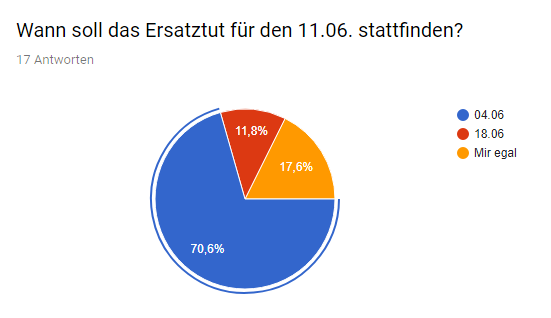
\includegraphics[scale=0.7]{pics/tut1/poll.png}
		\begin{itemize}
		\item Tut von 11.06 wird auf 04.06. verschoben
		\item ansonsten alles gleich (11:30-13:00, -119) 
	\end{itemize}
\end{frame}


	\subsection{Feedback 1. Übungsblatt}
	\begin{frame}
		\frametitle{1. Übungsblatt Statistik}
		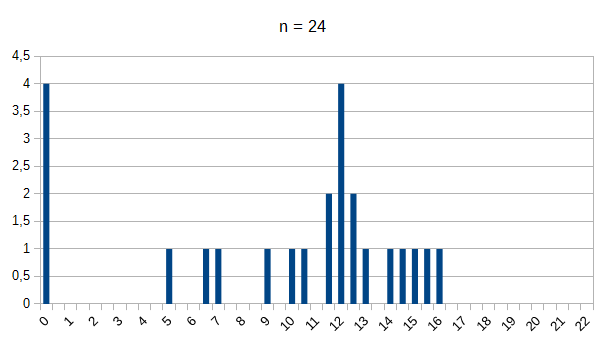
\includegraphics[scale=0.7]{./pics/tut1/statistics_ub1.png}
	\end{frame}
	
	\subsection{1. Übungsblatt - Fehler (Allgemein)}
	\begin{frame}
		\frametitle{Häufige Fehler}
		\begin{block}{Allgemein}
			generell ohne Abzug:
			\begin{itemize}
				\item gleiche Abgabe bei allen Aufgaben
			\end{itemize}
			\pause
			generell mit Abzug: (bis zu -2P)
			\begin{itemize}
				\item  CheckStyle nicht beachtet
				\item JavaDoc !(vollständig \&\& sinnvoll)
				\item Commits !(regelmäßig \&\& aussagekräftig)
			\end{itemize}
		\end{block}
	\end{frame}
	
	\subsection{1. Übungsblatt - Fehler (Aufgabe 1)}
	\begin{frame}
		\frametitle{Häufige Fehler}
		\begin{block}{Aufgabe 1 (Altsoftware vorbereiten)}
		\begin{itemize}
			\item vorgegebene .gitignore verwenden (mit IDE-Zeug), nicht nur target/ \pause
			\item fully.qualified.MainClass durch Paket-Struktur ersetzen (org.jis.Main)
		\end{itemize}
		\end{block}
	\end{frame}
	
	\subsection{1. Übungsblatt - Fehler (Aufgabe 2)}
	\begin{frame}
		\frametitle{Häufige Fehler}
		\begin{block}{Aufgabe 2 + 3 (Modultests + Testüberdeckung)}
			\begin{itemize}
				\item auch bei Drehung um 0$^{\circ}$  ist Überprüfung des Bildes nötig (Dimensionen + Pixel) \pause
				\item equals() reicht nicht aus, um Gleichheit der Bilder zu prüfen \pause 
				\item new File() erstellt kein File, sondern nur einen "'pointer"' auf einen Pfad (siehe File.createNewFile() oder File.mkdir()) \pause
				\item fügt Abhängigkeiten in die jmjrst.main-pom.xml ein, \textbf{nicht} in die von iMage \pause
				\item @Test(expected=XYException.class) nutzen \pause
				\item JUnit4 benutzen \pause
				\item nicht throws Exception angewöhnen \pause
				\item nicht Korrektheit der zu testenden Methoden annehmen \pause
				\item Stil: Konstanten für Pfade benutzen
			\end{itemize}
		\end{block}
	\end{frame}

%table of contents
\begin{frame}{Themenübersicht}
\tableofcontents
\end{frame}

\section{Wasserfallmodell}
	\subsection{Wasserfallmodell, ohne Grafik}
	\begin{frame}
		\frametitle{Wasserfallmodell}
		\begin{itemize}
			\item Was ist das? 
		\end{itemize}
	\end{frame}
	
	\subsection{Wasserfallmodell, mit Grafik}
	\begin{frame}
		\frametitle{Wasserfallmodell}
		\begin{itemize}
			\item \textcolor{red}{dokumentengetriebenes Prozessmodell} \pause
			\item mögliche Phasen der Softwareentwicklung \pause
		\end{itemize}
		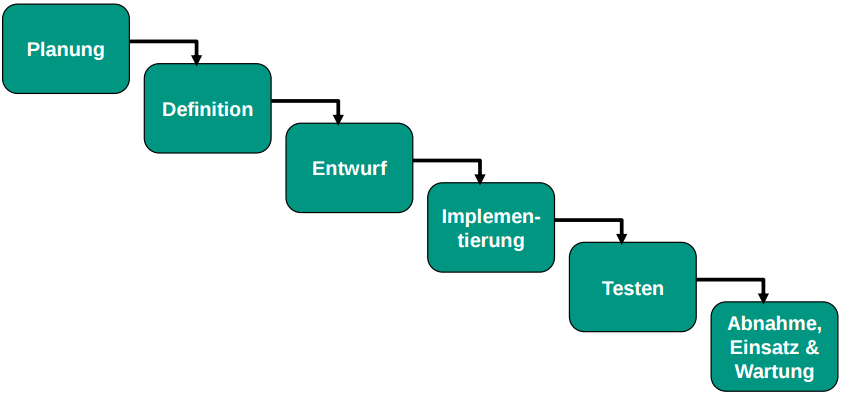
\includegraphics[scale=0.4]{./pics/tut1/waterfall_without-docs.png}
	\end{frame}
	
	\subsection{Wasserfallmodell, mit Grafik und Dokumenten}
	\begin{frame}
		\frametitle{Wasserfallmodell}
		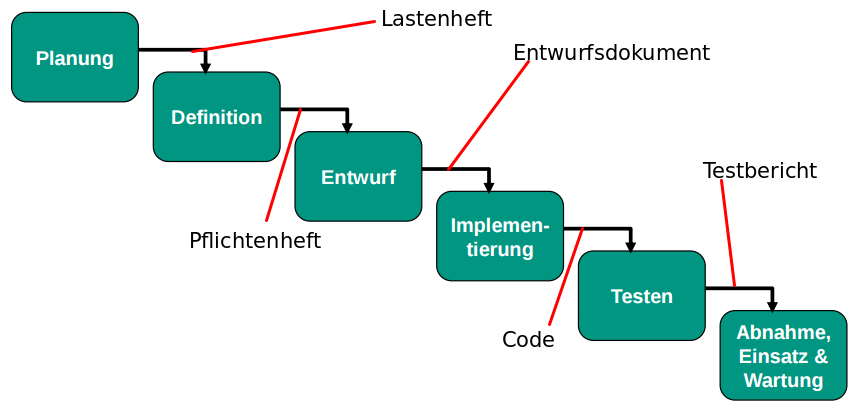
\includegraphics[scale=0.4]{./pics/tut1/waterfall_with-docs.png}
		\pause
		Dokumente für das 2. ÜB: 
		\begin{itemize}
			\item Lastenheft
			\item Durchführbarkeitsuntersuchung (weiteres Artefakt der Planung)
		\end{itemize}
	\end{frame}

\section{Durchführbarkeitsuntersuchung}
	\subsection{Welche Aspekte?}
	\begin{frame}
		\frametitle{Durchführbarkeitsuntersuchung}
		\begin{block}{Grundlegende Frage}
			Ist das Projekt in dem jeweiligen Szenario überhaupt durchführbar?
		\end{block}
		\begin{enumerate}
			\item \pause Fachlich \pause (softwaretechnisch leicht realisierbar?) \pause
			\item Alternativen \pause (lieber altes Projekt anpassen oder komplett neu entwickeln?) \pause
			\item Personell \pause (genug qualifizertes Personal?) \pause
			\item Risiken \pause (Gibt es Risiken? :D) \pause
			\item Ökonomisch \pause (wirtschaftlich? Termine?) \pause
			\item Rechtlich \pause (Datenschutz, Standards)
		\end{enumerate}
		\pause
		\begin{alertblock}{Fürs Übungsblatt}
			Denkt euch was (plausibles) aus!
		\end{alertblock}
	\end{frame}

\section{Lastenheft}
	\subsection{Lastenheft - Gliederung}
	\begin{frame}
		\frametitle{Lastenheft}
		\begin{block}{Grundlegende Aufgabe}
			Das Lastenheft sammelt die Anforderungen des Auftraggebers an den Auftragnehmer. Theoretisch vom Kunden geschrieben.
		\end{block}
		\begin{enumerate}
			\item \pause Zielbestimmung (grobe Beschreibung) \pause 
			\item Produkteinsatz (Für wen? Zielgruppe, Anwendungsbereich)\pause
			\item Funktionale Anforderungen (feingranular: Funktionen des Produkts)\pause 
			\item Produktdaten (Welche Daten speichern?)\pause
			\item Nichtfunktionale Anforderungen (Meta-Anforderungen: Zeit, Zuverlässigkeit)\pause 
			\item Systemmodelle
			\begin{itemize}
				\item Szenarien (spezielles Beispiel)
				\item Anwendungsfälle (allgemeiner Verwendungszweck)
			\end{itemize}
			\pause
			\item Glossar (technische Begriffe erklären)
		\end{enumerate}
	\end{frame}
	
	\subsection{Lastenheft - Unterschiede}
	\begin{frame}
		\frametitle{Begriffsklärung}
		\begin{block}{Zielbestimmung vs. Funktionale Anforderungen}
			\pause
			\begin{itemize}
				\item Zielbestimmung: allgemeine Beschreibung, was das Produkt können soll
				\item Funktionale Anforderungen: konkrete Auflistung von Funktionen
			\end{itemize}
		\end{block}
		\pause
		\begin{block}{Funktionale Anforderungen vs. Nichtfunktionale Anforderungen}
			\pause
			\begin{itemize}
				\item Funktionale Anforderungen: Funktionen des Produkts
				\item Nichtfunktionale Anforderungen: "'Meta"'-Eigenschaften des Produkts
			\end{itemize}
		\end{block}
		\pause
		\begin{block}{Zielbestimmung vs. Produkteinsatz}
			\pause
			\begin{itemize}
				\item Zielbestimmung: allgemeine Beschreibung, was das Produkt können soll
				\item Produkteinsatz: Rahmenbedingungen (Zielgruppe, Anwendungsbereiche)
			\end{itemize}
		\end{block}
	\end{frame}
	
\section{Pflichtenheft}
	\subsection{Pflichtenheft - Aufgabe}
	\begin{frame}
		\frametitle{Wozu ein Pflichtenheft?}
		\begin{block}{Grundlegende Aufgabe}
			Erweiterung des Lastenheftes, sodass exakt abgebildet ist \textbf{was} (noch nicht \textbf{wie}) zu implementieren ist. Vom Entwickler geschrieben.
		\end{block}
	\pause
		\begin{itemize}
			\item man kann es sich so merken
			\begin{itemize}
				\item erst werden uns \enquote{Lasten} vom Kunden auferlegt
				\item daraus generieren wir dann \enquote{Pflichten}
				\item \enquote{Pflichten} Grundlage für Entwurf
			\end{itemize}
		\end{itemize}
	\end{frame}
	
	\subsection{Pflichtenheft - Gliederung}
	\begin{frame}
		\frametitle{Pflichtenheft - Gliederung}
		\pause
		\begin{enumerate}
			\item Zielbestimmung  
			\item Produkteinsatz 
			\item \underline{\textbf{Produktumgebung}} (Hard-/Software in Einsatzumgebung)
			\item Funktionale Anforderungen 
			\item Produktdaten 
			\item Nichtfunktionale Anforderungen 
			\item \underline{\textbf{Globale Testfälle}} (\enquote{zu testende Abläufe})
			\item Systemmodelle
			\begin{itemize}
				\item Szenarien
				\item Anwendungsfälle
				\item \underline{\textbf{Objektmodelle}} $\implies$ UML-Klassendiagramme (heute)
				\item \underline{\textbf{Dynamische Modelle}} $\implies$ nächstes Mal
				\item \underline{\textbf{Benutzerschnittstelle}} $\implies$ Zeichnungen/Screenshots
			\end{itemize}
			\item Glossar 
		\end{enumerate}
	\end{frame}
	
	\subsection{Lastenheft - Unterschiede}
	\begin{frame}
		\frametitle{Begriffsklärung}
		\begin{block}{Produkteinsatz vs. Produktumgebung}
			\pause
			\begin{itemize}
				\item Produkteinsatz: Rahmenbedingungen (Zielgruppe, Anwendungsbereiche)
				\item Produktumgebung: Rahmenbedingungen bzgl. Software/Hardware
			\end{itemize}
		\end{block}
	\end{frame}
	
	\subsection{Quiz}
	\begin{frame}
		\frametitle{Quiz (Ankreuzaufgaben aus Klausuren)}
		Wahr oder falsch?
		\begin{itemize}
			\item Das Lastenheft ist eine Verfeinerung des Pflichtenheftes. \pause \colorbox{red}{falsch} \pause
			\item Das Lastenheft ist das Ergebnis der Planungsphase. \pause \colorbox{green}{wahr} \pause
			\item Nicht-funktionale Eigenschaften beschreiben, was das Produkt nicht tun sollte. \pause \colorbox{red}{falsch} \pause 
			\item Das Pflichtenheft beschreibt nur, was zu implementieren ist und nicht wie. \pause \colorbox{green}{wahr} \pause 
			\item Nicht-funktionale Anforderungen sind sowohl Teil des Pflichtenhefts als auch des Lastenhefts. \pause \colorbox{green}{wahr}
		\end{itemize}
		
	\end{frame}

\section{UML-Klassendiagramm}
	\subsection{UML? Kann man das essen?}
	\begin{frame}
		\frametitle{UML? Kann man das essen?}
		\begin{itemize}
			\item UML = \textbf{U}nified \textbf{M}odeling \textbf{L}anguage
			\item grafische Modellierungssprache, strenge Syntax
		\end{itemize}
		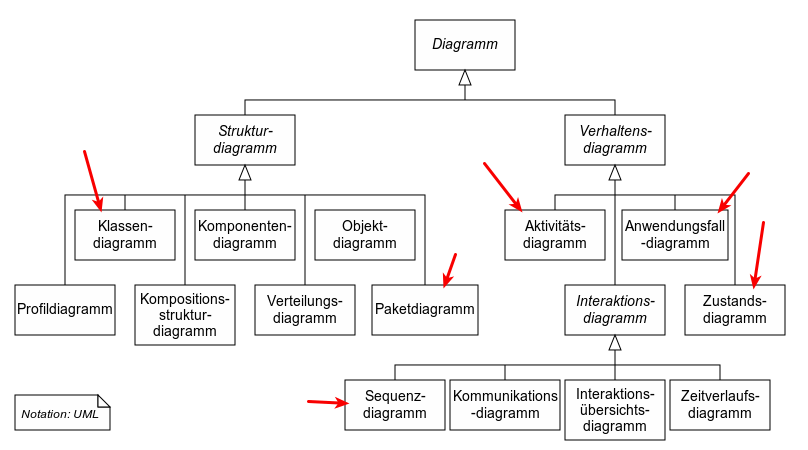
\includegraphics[scale=0.35]{./pics/tut1/uml_diagrams.png}
	\end{frame}	

	\begin{frame}[fragile]{UML-Klassendiagramm: Syntax}
	\begin{columns}
		\begin{column}{0.25\textwidth}
				\begin{tikzpicture}
				\centering
			\umlclass[name=classname]{Name der Klasse}{Attribute}{Methoden}
			\end{tikzpicture}
		\end{column}%
		\begin{column}{0.75\textwidth}
			\begin{itemize}
				\item Klassenname
				\begin{itemize}
					\item keine spezielle Syntax
					\item einfach Namen hinschreiben
				\end{itemize}
				\item Attribute
				\begin{itemize}
					\item \begin{verbatim}<modifier><name>:<type>\end{verbatim} 
				\end{itemize} 
				\item Methoden
				\begin{itemize}
					\item \begin{verbatim}<modifier><name>(<parameters>):<type>\end{verbatim}
					\item \verb|<parameters>|
					\begin{itemize}
						\item kann leer sein
						\item oder komma-getrennte Liste von \verb|<name>:<type>|
					\end{itemize}
					\item falls Rückgabe void, \verb|:<type>| weglassen
					
				\end{itemize} 
			\item statische Methoden und Attribute unterstreichen
			\end{itemize}
		\end{column}
	\end{columns}
\end{frame}

\begin{frame}{Modifier}
	\begin{itemize}
		\item UML
		\begin{itemize}
			\item -
			\begin{itemize}
				\item private
				\item von Instanzen derselben Klasse sichtbar (\textcolor{red}{aber von allen!})
			\end{itemize}
			\item \#
			\begin{itemize}
				\item protected (wie in Java)
				\item von Instanzen derselben Klasse, aller Unterklassen und Instanzen aus dem gleichen Paket sichtbar
			\end{itemize}
			\item +
			\begin{itemize}
				\item public (wie in Java)
				\item von Instanzen jeder Klasse sichtbar
			\end{itemize}
			\item falls nichts angegeben implizit public
		\end{itemize}
	\end{itemize}
\end{frame}

\begin{frame}{Beispiel}
\begin{figure}
	\centering
	\begin{tikzpicture}
		\umlclass[name=classname]{Hund}{- name: String\\
		- rasse: Rasse\\
		- gewicht: int}{
		+ wiegen(): int\\
		+ streicheln() \\
		+ streicheln(intensität: int, ausruf: String)\\
		+ füttern(ration: Nahrung)}
	\end{tikzpicture}
\end{figure}
\end{frame}
	
	\subsection{UML-Klassendiagramm (1)}
	\begin{frame}
		\frametitle{Vererbung}
		\begin{figure}
					\centering
			\begin{tikzpicture}
			\pgfsetlayers{connections,main}
				\umlclass[y=4,name=classname]
				{ParentClass}
				{+publicString: String \\
				-privateInt: int\\
				\#protectedDouble: double}
				{
				\umlstatic{+staticMethod()}\\
				+publicMethod(): String\\
				-privateMethod(): int\\
				\#protectedMethod(param: String): double
				}
			
				\umlemptyclass[y=0, name=classname]{ChildClass}
				
				\umlinherit{ChildClass}{ParentClass}
			\end{tikzpicture}
		\end{figure}
	\end{frame}
	
	\subsection{UML-Klassendiagramm (2)}
	\begin{frame}
		\frametitle{Interface}
				\begin{figure}
			\centering
			\begin{tikzpicture}
			\pgfsetlayers{connections,main}
			\umlclass[y=4,name=classname, type=interface]{NiceInterface}
			{}
			{
				+pleaseRealizeMe()
			}
			
			\umlclass[y=0, name=classname]{ImplementingClass}{}{+pleaseRealizeMe()}
			
			\umlimpl{ImplementingClass}{NiceInterface}
			\end{tikzpicture}
		\end{figure}
	\end{frame}
	
	\subsection{UML-Klassendiagramm (3)}
	\begin{frame}
		\frametitle{Abstrakte Klassen}
				\begin{figure}
			\centering
			\begin{tikzpicture}
			\pgfsetlayers{connections,main}
			\umlclass[y=3,name=classname,type=abstract]
			{AbstractClass}
			{}
			{
				+regularMethod(): String\\
				\umlvirt{+abstractMethod(): int}
			}
			
			\umlclass[y=0, name=classname]{ChildClass}{}{+abstractMethod(): int}
			
			\umlinherit{ChildClass}{AbstractClass}
			\end{tikzpicture}
		\end{figure}
	\end{frame}

	\begin{frame}
\frametitle{Abstrakte Klassen: Abgaben}
\begin{figure}
	\centering
	\begin{tikzpicture}
	\pgfsetlayers{connections,main}
	\umlclass[y=3,name=classname,tags={abstract}]
	{AbstractClass}
	{}
	{
		+regularMethod(): String\\
		+abstractMethod(): int \{abstract\}
	}
	
	\umlclass[y=0, name=classname]{ChildClass}{}{+abstractMethod(): int}
	
	\umlinherit{ChildClass}{AbstractClass}
	\end{tikzpicture}
\end{figure}
\begin{itemize}
	\item für Übungsblätter und Klausur
	\begin{itemize}
		\item kursiv nicht erkennbar, stattdessen \texttt{\{abstract\}} verwenden
		\item laut VL unter Klassenname, hinter Methode
	\end{itemize}
\end{itemize}
\end{frame}
	
	\subsection{UML-Klassendiagramm (4)}
	\begin{frame}
		\frametitle{Assoziationen}
		\begin{figure}
			\centering
			\begin{tikzpicture}
			\pgfsetlayers{connections,main}
			\umlclass[x=0,name=classname]
			{Firma}
			{angestellte: List$<$Person$>$}
			{}
			
			\umlclass[
			x=6, name=classname]{Person}{arbeitgeber: Firma}{}
			
			\end{tikzpicture}
		\end{figure}
	\pause
		\begin{alertblock}{Probleme}
			\begin{itemize}
				\item List$<$X$>$ ist Java-Syntax und schreibt Datenstruktur vor
				\item Beziehungen sollen direkt ersichtlich werden
				\item Faustregel: nur primitive Typen als Attribute hinschreiben
			\end{itemize}
		\end{alertblock}
				\begin{figure}
			\centering
			\begin{tikzpicture}
			\pgfsetlayers{connections,main}
			\umlclass[x=0,name=classname]
			{Firma}
			{}
			{}
			
			\umlclass[
			x=8, name=classname]{Person}{}{}
			
			\umlassoc[arg1=Arbeitgeber, arg2=Arbeitnehmer, mult1=0..1, mult2=*, pos1=0, pos2=1, align1=left, align2=right]{Firma}{Person}
			\end{tikzpicture}
		\end{figure}
	\end{frame}
	
	\subsection{UML-Klassendiagramm (5)}
	\begin{frame}
		\frametitle{Aggregation und Komposition}
		\begin{itemize}
			\item Aggregation = Teil-Ganzes-Beziehung
		\end{itemize}
			\begin{figure}
			\centering
			\begin{tikzpicture}
			\pgfsetlayers{connections,main}
			\umlclass[x=0,name=classname]
			{Auto}
			{}
			{}
			
			\umlclass[
			x=8, name=classname]{Rad}{}{}
			
			\umlaggreg[arg1=1, arg2=4, pos1=0, pos2=1, align1=left, align2=right, thick]{Auto}{Rad}
			\end{tikzpicture}
		\end{figure}
	\pause
		\begin{itemize}
			\item Komposition: Aggregation, aber Teil kann ohne Ganzes nicht existieren
			\begin{itemize}
				\item wenn ganzes gelöscht wird, dann auch Teile!
			\end{itemize}
		\end{itemize}
				\begin{figure}
		\centering
		\begin{tikzpicture}
		\pgfsetlayers{connections,main}
		\umlclass[x=0,name=classname]
		{Rechnung}
		{}
		{}
		
		\umlclass[
		x=8, name=classname]{Rechnungsposten}{}{}
		
		\umlcompo[arg1=1, arg2=1..*, pos1=0, pos2=1, align1=left, align2=right,thick]{Rechnung}{Rechnungsposten}
		\end{tikzpicture}
	\end{figure}
\end{frame}

	\subsection{UML-Warmup-Aufgabe}
	\begin{frame}
		\frametitle{Klassischer Aufgabentyp}
		\begin{exampleblock}{Text $\implies$ UML-Klassendiagramm}
			Jeder Student hat eine Matrikelnummer und einen Namen. Ein fauler Student ist ein Student, der schlafen kann. Er hat dazu ein Bett. Ein fleißiger Student hingegen, kann lernen und hat dazu einen Computer, der aus Bauteilen besteht.
		\end{exampleblock}
	\pause
	\textcolor{red}{UML-Diagramm?}
\end{frame}

	\subsection{UML-Warmup-Aufgabe2}
	\begin{frame}
	\frametitle{Klassischer Aufgabentyp}
	\begin{exampleblock}{Text $\implies$ UML-Klassendiagramm}
		Jeder \textcolor{red}{Student} hat eine Matrikelnummer und einen Namen. Ein fauler Student \textcolor{red}{ist ein} Student, der schlafen kann. Er \textcolor{red}{hat} dazu ein Bett. Ein fleißiger Student hingegen, kann lernen und \textcolor{red}{hat} dazu einen \textcolor{red}{Computer}, der aus \textcolor{red}{Bauteilen} \textcolor{red}{besteht}.
	\end{exampleblock}
	\textcolor{red}{Schlüsselwörter!}
\end{frame}
	
	\subsection{UML-Klausuraufgabe(1)}
	\begin{frame}
		\frametitle{Klausuraufgabe SS09}
		\textit{Modellieren Sie das Szenario möglichst vollständig als UML-Klassendiagramm. Modellieren Sie keine Methoden. Geben Sie Attribute, Multiplizitäten, Restriktionen, Assoziationsnamen sowie Rollen an.} \linebreak
		Ein Fachwerkhaus besteht aus 5 bis 10 Holzstämmen, 200 bis 400 Lehmziegeln sowie 1.000 bis 2.000 Nägeln. Jedes Baumaterial, egal ob Holzstamm, Lehmziegel oder Nagel, ist Bestandteil in genau einem Fachwerkhaus. Jedes Fachwerkhaus hat eine bestimmte Anzahl an Zimmern und Stockwerken. Für den Bau eines Fachwerkhauses ist mindestens ein Zimmermann zuständig, welcher einen Namen sowie einen individuellen Stundenlohn besitzt. Zum Bau des Fachwerkhauses verwendet jeder Zimmermann sein eigenes Werkzeug, bestehend aus genau einem Hammer sowie genau einer Säge. Jeder Zimmermann kann an maximal einem Fachwerkhaus gleichzeitig bauen. 
	\end{frame}
	
	\subsection{UML-Klausuraufgabe(2)}
	\begin{frame}
		\frametitle{Musterlösung}
		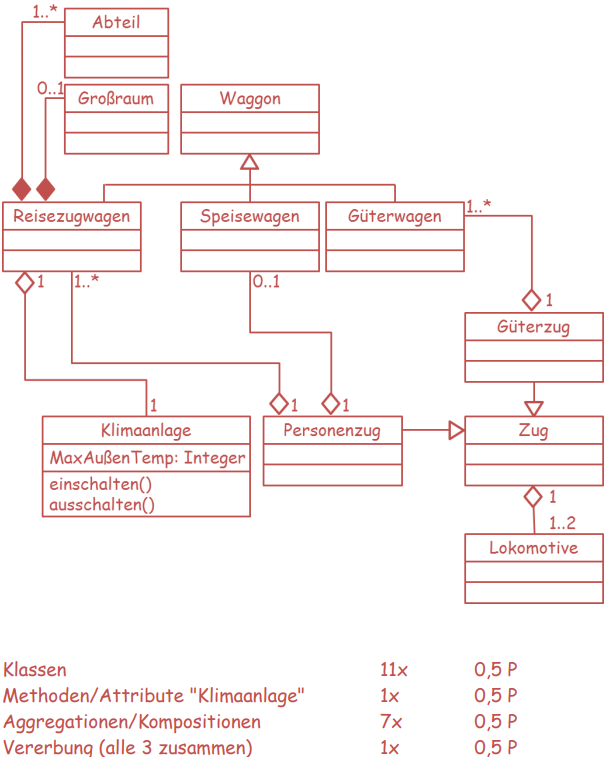
\includegraphics[scale=0.48]{./pics/tut1/solution.png}
	\end{frame}
		
		
\section{\LaTeX}
	\subsection{Basics}
	\begin{frame}
		\frametitle{\LaTeX - Basics}
		\begin{itemize}
			\item auf dem Blatt müsst ihr \LaTeX  ~ für die Dokumente benutzen
			\item nicht wie z.B. Word WYSIWYG, sondern WYSIWYAF / WYSIWYM
			\item wird euch an der Uni immer wieder begegnen, oft Pflicht
			\pause
			\item Vorteile:
			\begin{itemize}
				\item gut versionierbar
				\item leicht Formeln erstellbar
				\item nach Eingewöhnung recht intuitiv (vergleichbar mit HTML)
				\item multifunktional (Dokumente, Präsentationen, \dots)
			\end{itemize}
			\pause
			\item Nachteile:
			\begin{itemize}
				\item Einarbeitung notwendig :(
			\end{itemize}
		\end{itemize}
	\end{frame}
	
	\subsection{Installation}
	\begin{frame}
		\frametitle{\LaTeX - Installation}
		Installation einer Distribution notwendig, z.B.:
		\begin{itemize}
			\item  MiKTeX für Windows
			\item TeX Live für Linux, Mac, Windows
		\end{itemize}
		\pause
		Editoren machen das Schreiben von \LaTeX -Dokumenten angenehmer
		\begin{itemize}
			\item Texmaker
			\item TeXstudio (erweiterter Texmaker, mein Favorit)
			\item TeXclipse (Plugin für Eclipse)
			\item \dots
		\end{itemize}
	\end{frame}
	
	\subsection{Beispiel}
	\begin{frame}
		\frametitle{\LaTeX - Dokumentaufbau}
		\begin{itemize}
			\item Präambel: Includes von Paketen
			\begin{itemize}
				\item $\backslash$documentclass\{Klasse\} (z.B. book, letter)
				\item $\backslash$usepackage[option1, option2,..]\{Paket\}
			\end{itemize}
			\pause
			\item Inhalt: Text setzen 
			\begin{itemize}
				\item Struktur: part, (chapter), section, subsection, subsubsection
				\item Auflistungen: $\backslash$begin\{itemize\} $\backslash$item Hello World! $\backslash$end\{itemize\}
				\item Bilder: $\backslash$includegraphics$[scale=0.8]$\{PfadZumBild\}
			\end{itemize}
			\pause
		\end{itemize}
		\huge \centering \textcolor{red}{Beispiel!}
	\end{frame}
		
\section{Tipps}
	\subsection{Tipps}
	\begin{frame}
		\frametitle{Tipps - 2. Übungsblatt}
		\begin{small}
			\begin{exampleblock}{Aufgabe 1 + 3: Lastenheft + Durchführbarkeitsuntersuchung}
				\begin{itemize}
					\item lasst euch was (sinnvolles) einfallen
					\item benutzt \LaTeX
				\end{itemize}
			\end{exampleblock}
			\pause
			\begin{exampleblock}{Aufgabe 2: Klassendiagramme}
				\begin{itemize}
					\item achtet auf Schlüsselwörter ("'ist ein"', "'enthält ein"', "'besteht aus"',\dots)
				\end{itemize}
			\end{exampleblock}
			\pause
			\begin{exampleblock}{Aufgabe 4 + 5: Shutterpile}
				\begin{itemize}
					\item an einigen Stellen sind Aufgaben etwas vage
					\linebreak $\implies$ überlegt euch, was Sinn macht
					\item Zusammenhang der Klassen unklar? Vielleicht hilft Diagramm
				\end{itemize}
			\end{exampleblock}
		\end{small}
	\end{frame}
	
	\subsection{Abgabe}
	\begin{frame}
		\frametitle{Denkt dran!}
		\begin{alertblock}{Abgabe}
			\begin{itemize}
				\item Deadline am 16.5 um 12:00
				\item Dokumente ausdrucken
				\item Klassendiagramme handschriftlich
			\end{itemize}
		\end{alertblock}
	\end{frame}
		
	\begin{frame}
		\frametitle{Bis dann! (dann := 22.05.18)}
		\centering
		
\includegraphics[scale=0.86]{./comics/geek_and_poke_javadoc.jpg}
	\end{frame}

\end{document}
